\begin{figure}[ht]
\centering\fbox{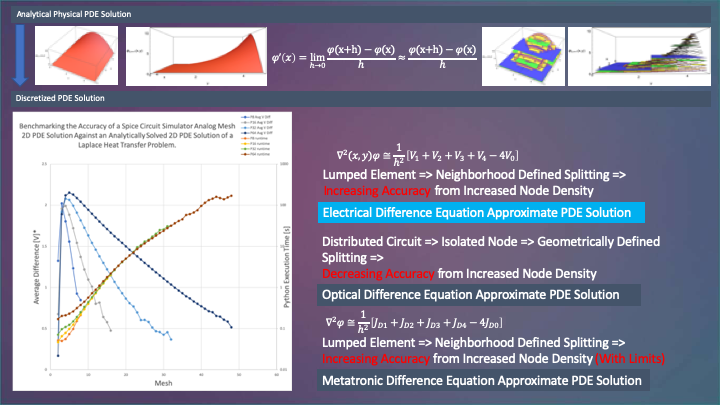
\includegraphics[height=3in, width=5.5in]{figures/figures1/03a_elec_accuracy.png}}
\caption{Electronic analog exhibits lumped element, neighborhood defined splitting, and increased accuracy from increased node density.}
\label{fig:1_03a_elec_accuracy}
\end{figure}
 
\par When transitioning from analytical to discrete Solutions, discretization error is the principal source of error in the finite difference method employed in all of the discrete information processing techniques that are discussed in the thesis. For a one dimensional problem the discretization error of $\psi$ can be defined in terms of its derivative. This spatial change is defined by $h$, and shown at the top of Figure \ref{fig:1_03a_elec_accuracy}, which is finitely small and the removal of the limit creates the approximation which is defined as the discretization error. For a dense discretized solution where the number of nodes $n$ approaches infinity and acts like a continuous solution we expect the accuracy of the overall solution to increase. One can see accuracy improvement electronically as the electronic analog exhibits lumped element, neighborhood defined splitting, and increased accuracy from increased node density as shown in Figure \ref{fig:1_03a_elec_accuracy}.

\begin{figure}[ht]
\centering\fbox{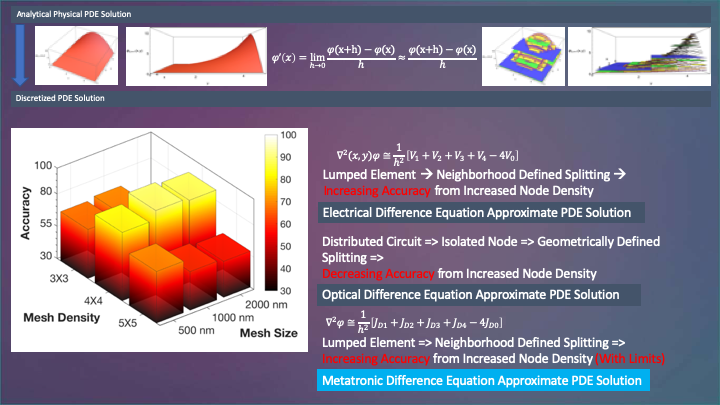
\includegraphics[height=3in, width=5.5in]{figures/figures1/03b_mt_accuracy.png}}
\caption{The metatronic circuit exhibits lumped element, neighborhood defined splitting, and therefore increasing accuracy from increased node density all at at a smaller operational wavelength than the electrical analog.}
\label{fig:1_03b_mt_accuracy.png}
\end{figure} 

\par The details of geometric optical splitting utilized in the photonics mesh is explored by my colleagues Shuai Sun and Engin Kayraklioglu who will give a deep explanation in their dissertations. However due to the distributed circuit, isolated node, and therefore geometrically defined splitting behavior, phonically one expects decreasing accuracy from increased node density. This does not mean that a photonic implementation cannot provide a useful approximate solution, but the photonic architecture needs to compensate for this negative effect. On a positive note, the metatronic circuit exhibits lumped element, neighborhood defined splitting and therefore increasing accuracy from increased node density all at at a smaller wavelength than the electrical analog as shown in Figure \ref{fig:1_03b_mt_accuracy.png}.
 

